\documentclass[a4paper,10pt,abstracton]{scrartcl}

\usepackage[margin=2.5cm]{geometry}
\usepackage{graphicx}
\usepackage[UKenglish]{babel}
\usepackage{csquotes}
\usepackage[style=numeric,citestyle=numeric,backend=biber,sorting=none,doi=false,url=false]{biblatex}
\usepackage{float}
\usepackage[export]{adjustbox}
\usepackage[T1]{fontenc}
\usepackage{lmodern}
\usepackage{todonotes}
\usepackage[labelsep=period,font=small,labelfont=bf,format=plain]{caption}
\usepackage[group-separator={,}]{siunitx}
\usepackage{booktabs}
\usepackage{pdflscape}
\usepackage{tablefootnote}

\title{The genetic architecture of target-site resistance to DDT and
  pyrethroids in the malaria vectors \emph{Anopheles gambiae} and
  \emph{Anopheles coluzzii}}

\subtitle{DRAFT}

\author{
	Chris S. Clarkson
	\and 
	Alistair Miles
	\and
	Nicholas J. Harding
        \and
        ...
	\and
	Dominic Kwiatkowski
	\and
	Martin Donnelly
	\and
	The Anopheles gambiae 1000 Genomes Consortium
} 
%\date{January 21, 1994}

\begin{document}

\maketitle

\begin{abstract}

%%
TODO

\end{abstract}

\section*{Introduction}

The malaria vectors \emph{Anopheles gambiae} and \emph{Anopheles
  coluzzii} are evolving insecticide resistance asdlkj dsalkj daslkjd
aslkjdas lkadsj lkadsj adslkj adslkja dslkadsj lkadsj lkasd jlkads
jlkadsj lkads jlakds alksdj asdlk jasdlk adslk jadslkj adslkj adslkj
adslkj adslkj adslk jasd

This is the second paragraph of the introduction, asdlkjio weipo
ewrpoi ewrpoi rwepoi werpoiwre poi rewpoi rwepoi erwpoi rewpoi rwepoi
rwepoi rwepoi rewpo iwrepoi rwepoi wrepoi wrepoi rwpeo irwpo irwepoi
rwepo ipoewi rpow ierwe

Third paragraph zcx,m ncxz,mxczn ,mxczn,mxcz n,mcnxz ,mxczn ,mz ncx,m
zcxn

Fourth paragraph asdlkj dsakljdsalkj dsalkj daslkj daslkj dsalkj
daslkj sda

TODO

\section*{Results}

Let's add some results qweoi qewoiewqoip peqwpoi ewqpoi ewqpoieqwipo
ewqipo eqwpio eqwipo ewqoip ewqoip ewqiop eqw

Isn't Figure \ref{fig:demo} interesting! Table \ref{table:demo} is
pretty interesting too.

\begin{landscape}
\begin{table}[h]
  \small
  \centering
  
\begin{tabular}{lllrrrrrrrrrrr}
\toprule
\multicolumn{3}{c}{Mutation} &
\multicolumn{9}{c}{Population allele frequency (\%)} &
\multicolumn{2}{c}{LD ($D'$)} \\
\cmidrule(r){1-3}
\cmidrule(r){4-12}
\cmidrule(r){13-14}
Position\tablefootnote{Position relative to AgamP3 reference sequence, chromosome arm 2L.} & 
\emph{Ag}\tablefootnote{Codon numbering according to transcript \texttt{AGAP004707-RA} in geneset AgamP4.4.} & 
\emph{Md}\tablefootnote{Codon numbering according to @@TODO.} & 
AO\emph{Ac} & 
BF\emph{Ac} & 
GN\emph{Ag} & 
BF\emph{Ag} & 
CM\emph{Ag} & 
GA\emph{Ag} & 
UG\emph{Ag} & 
KE & 
GW & 
\texttt{L995F} & 
\texttt{L995S} \\
\midrule

\texttt{2,390,177 G>A} & \texttt{R254K} & NA & 0 & 0 & 0 & 0 & 32 & 21 & 0 & 0 & 0 & NA & NA \\

\texttt{2,391,228 G>C} & \texttt{V402L} & NA & 0 & 7 & 0 & 0 & 0 & 0 & 0 & 0 & 0 & NA & NA \\

\texttt{2,391,228 G>T} & \texttt{V402L} & NA & 0 & 7 & 0 & 0 & 0 & 0 & 0 & 0 & 0 & NA & NA \\

\texttt{2,399,997 G>C} & \texttt{D466H} & NA & 0 & 0 & 0 & 0 & 7 & 0 & 0 & 0 & 0 & NA & NA \\

\texttt{2,400,071 G>A} & \texttt{M490I} & NA & 0 & 0 & 0 & 0 & 0 & 0 & 0 & 18 & 0 & NA & NA \\

\texttt{2,400,071 G>T} & \texttt{M490I} & NA & 0 & 0 & 0 & 0 & 0 & 0 & 0 & 0 & 0 & NA & NA \\

\texttt{2,416,980 C>T} & \texttt{T791M} & NA & 0 & 1 & 13 & 14 & 0 & 0 & 0 & 0 & 0 & NA & NA \\

\texttt{2,422,651 T>C} & \texttt{L995S} & NA & 0 & 0 & 0 & 0 & 15 & 64 & 100 & 76 & 0 & NA & NA \\

\texttt{2,422,652 A>T} & \texttt{L995F} & NA & 86 & 85 & 100 & 100 & 53 & 36 & 0 & 0 & 0 & NA & NA \\

\texttt{2,424,384 C>T} & \texttt{A1125V} & NA & 9 & 0 & 0 & 0 & 0 & 0 & 0 & 0 & 0 & NA & NA \\

\texttt{2,425,077 G>A} & \texttt{V1254I} & NA & 0 & 0 & 0 & 0 & 0 & 0 & 0 & 0 & 5 & NA & NA \\

\texttt{2,429,617 T>C} & \texttt{I1527T} & NA & 0 & 14 & 0 & 0 & 0 & 0 & 0 & 0 & 0 & NA & NA \\

\texttt{2,429,745 A>T*} & \texttt{N1570Y} & NA & 0 & 26 & 10 & 22 & 6 & 0 & 0 & 0 & 0 & NA & NA \\

\texttt{2,429,897 A>G} & \texttt{E1597G} & NA & 0 & 0 & 6 & 4 & 0 & 0 & 0 & 0 & 0 & NA & NA \\

\texttt{2,429,915 A>C} & \texttt{K1603T} & NA & 0 & 5 & 0 & 0 & 0 & 0 & 0 & 0 & 0 & NA & NA \\

\texttt{2,430,424 G>T} & \texttt{A1746S} & NA & 0 & 0 & 11 & 13 & 0 & 0 & 0 & 0 & 0 & NA & NA \\

\texttt{2,430,817 G>A} & \texttt{V1853I} & NA & 0 & 0 & 8 & 5 & 0 & 0 & 0 & 0 & 0 & NA & NA \\

\texttt{2,430,863 T>C} & \texttt{I1868T} & NA & 0 & 0 & 18 & 25 & 0 & 0 & 0 & 0 & 0 & NA & NA \\

\texttt{2,430,880 C>T} & \texttt{P1874S} & NA & 0 & 21 & 0 & 0 & 0 & 0 & 0 & 0 & 0 & NA & NA \\

\texttt{2,430,881 C>T} & \texttt{P1874L} & NA & 0 & 7 & 45 & 26 & 0 & 0 & 0 & 0 & 0 & NA & NA \\

\texttt{2,431,061 C>T} & \texttt{A1934V} & NA & 0 & 12 & 0 & 0 & 0 & 0 & 0 & 0 & 0 & NA & NA \\

\texttt{2,431,079 T>C} & \texttt{I1940T} & NA & 0 & 4 & 0 & 0 & 7 & 0 & 0 & 0 & 0 & NA & NA \\

\bottomrule
\end{tabular}

  \caption{\textbf{Non-synonymous mutations in the voltage-gated
      sodium channel gene}. All mutations are at 5\% frequency or
    above in one or more of the 9 Ag1000G phase 1 populations, with
    the exception of \texttt{2,400,071 G>T} which is at 0.4\%
    frequency in the CM\emph{Ag} population but is included because
    another mutation (\texttt{2,400,071 G>A}) is found at the same
    position causing the same amino acid substitution
    (\texttt{M490I}). Substitutions marked with an asterisk (*) failed
    conservative variant filters applied genome-wide in the Ag1000G
    phase 1 AR3 callset, but appeared sound on manual inspection of
    read alignments.}
  \label{table:variants_missense}
\end{table}
\end{landscape}

\begin{figure}[t!]
  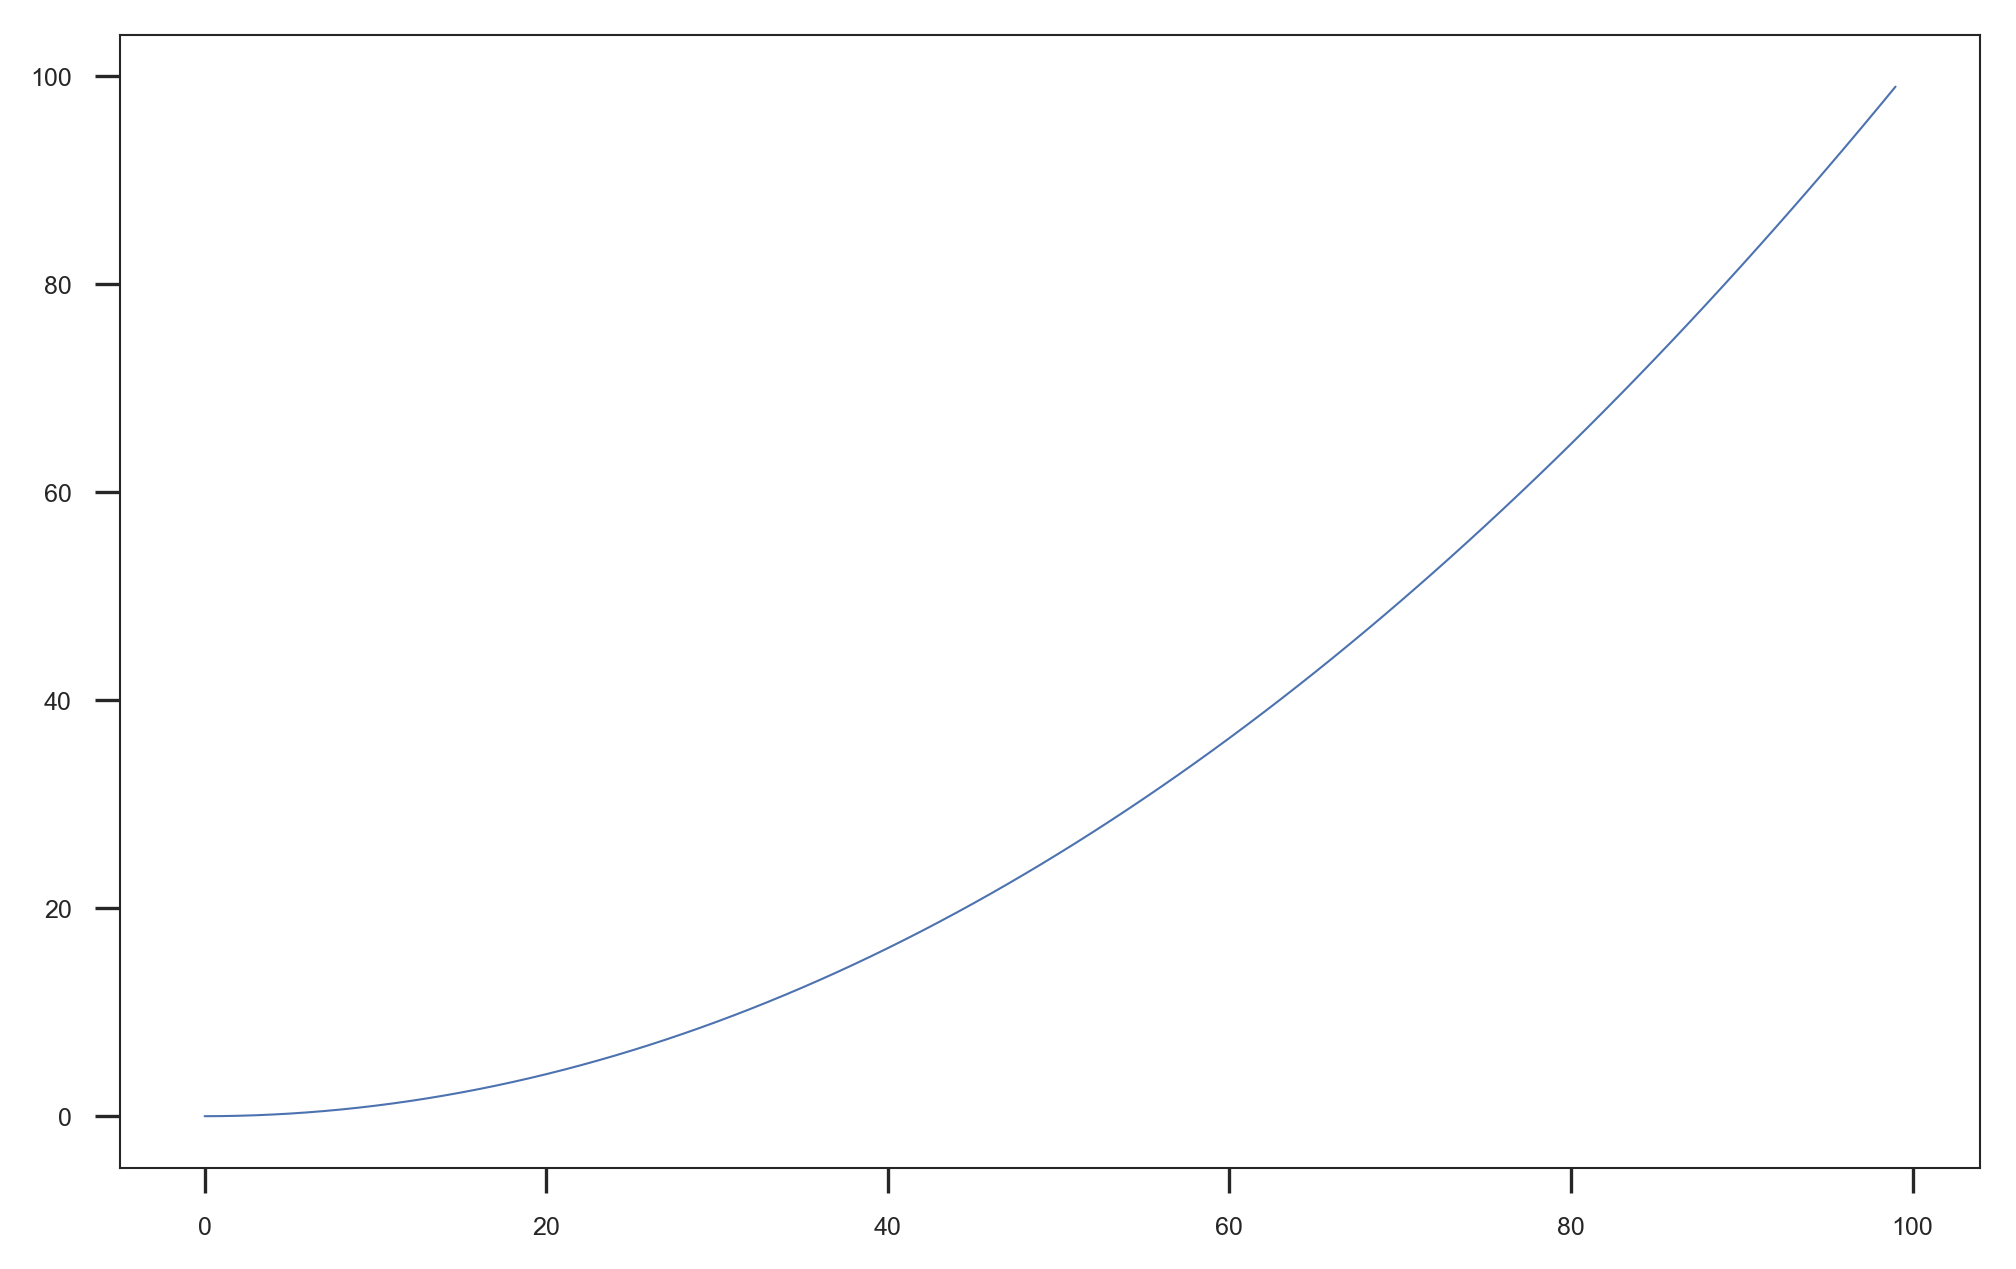
\includegraphics[width=1.1\linewidth,center]{artwork/demo.png}
  \caption{Demo figure.}
  \label{fig:demo}
\end{figure}

TODO

\begin{table}[h]
  \centering
  
\begin{tabular}{rll}
\toprule
Foo & Bar & Baz \\
\midrule

1 & a & True \\

2 & b & False \\

\bottomrule
\end{tabular}

  \caption{This is a table.}
  \label{table:demo}
\end{table}

\section*{Discussion}

TODO

\section*{Methods}

TODO

\end{document}
